
\section{Mô hình sinh cử chỉ}

%\begin{frame}{Tổng quan về bài toán}
%%	\begin{figure}
%%		\centering
%%		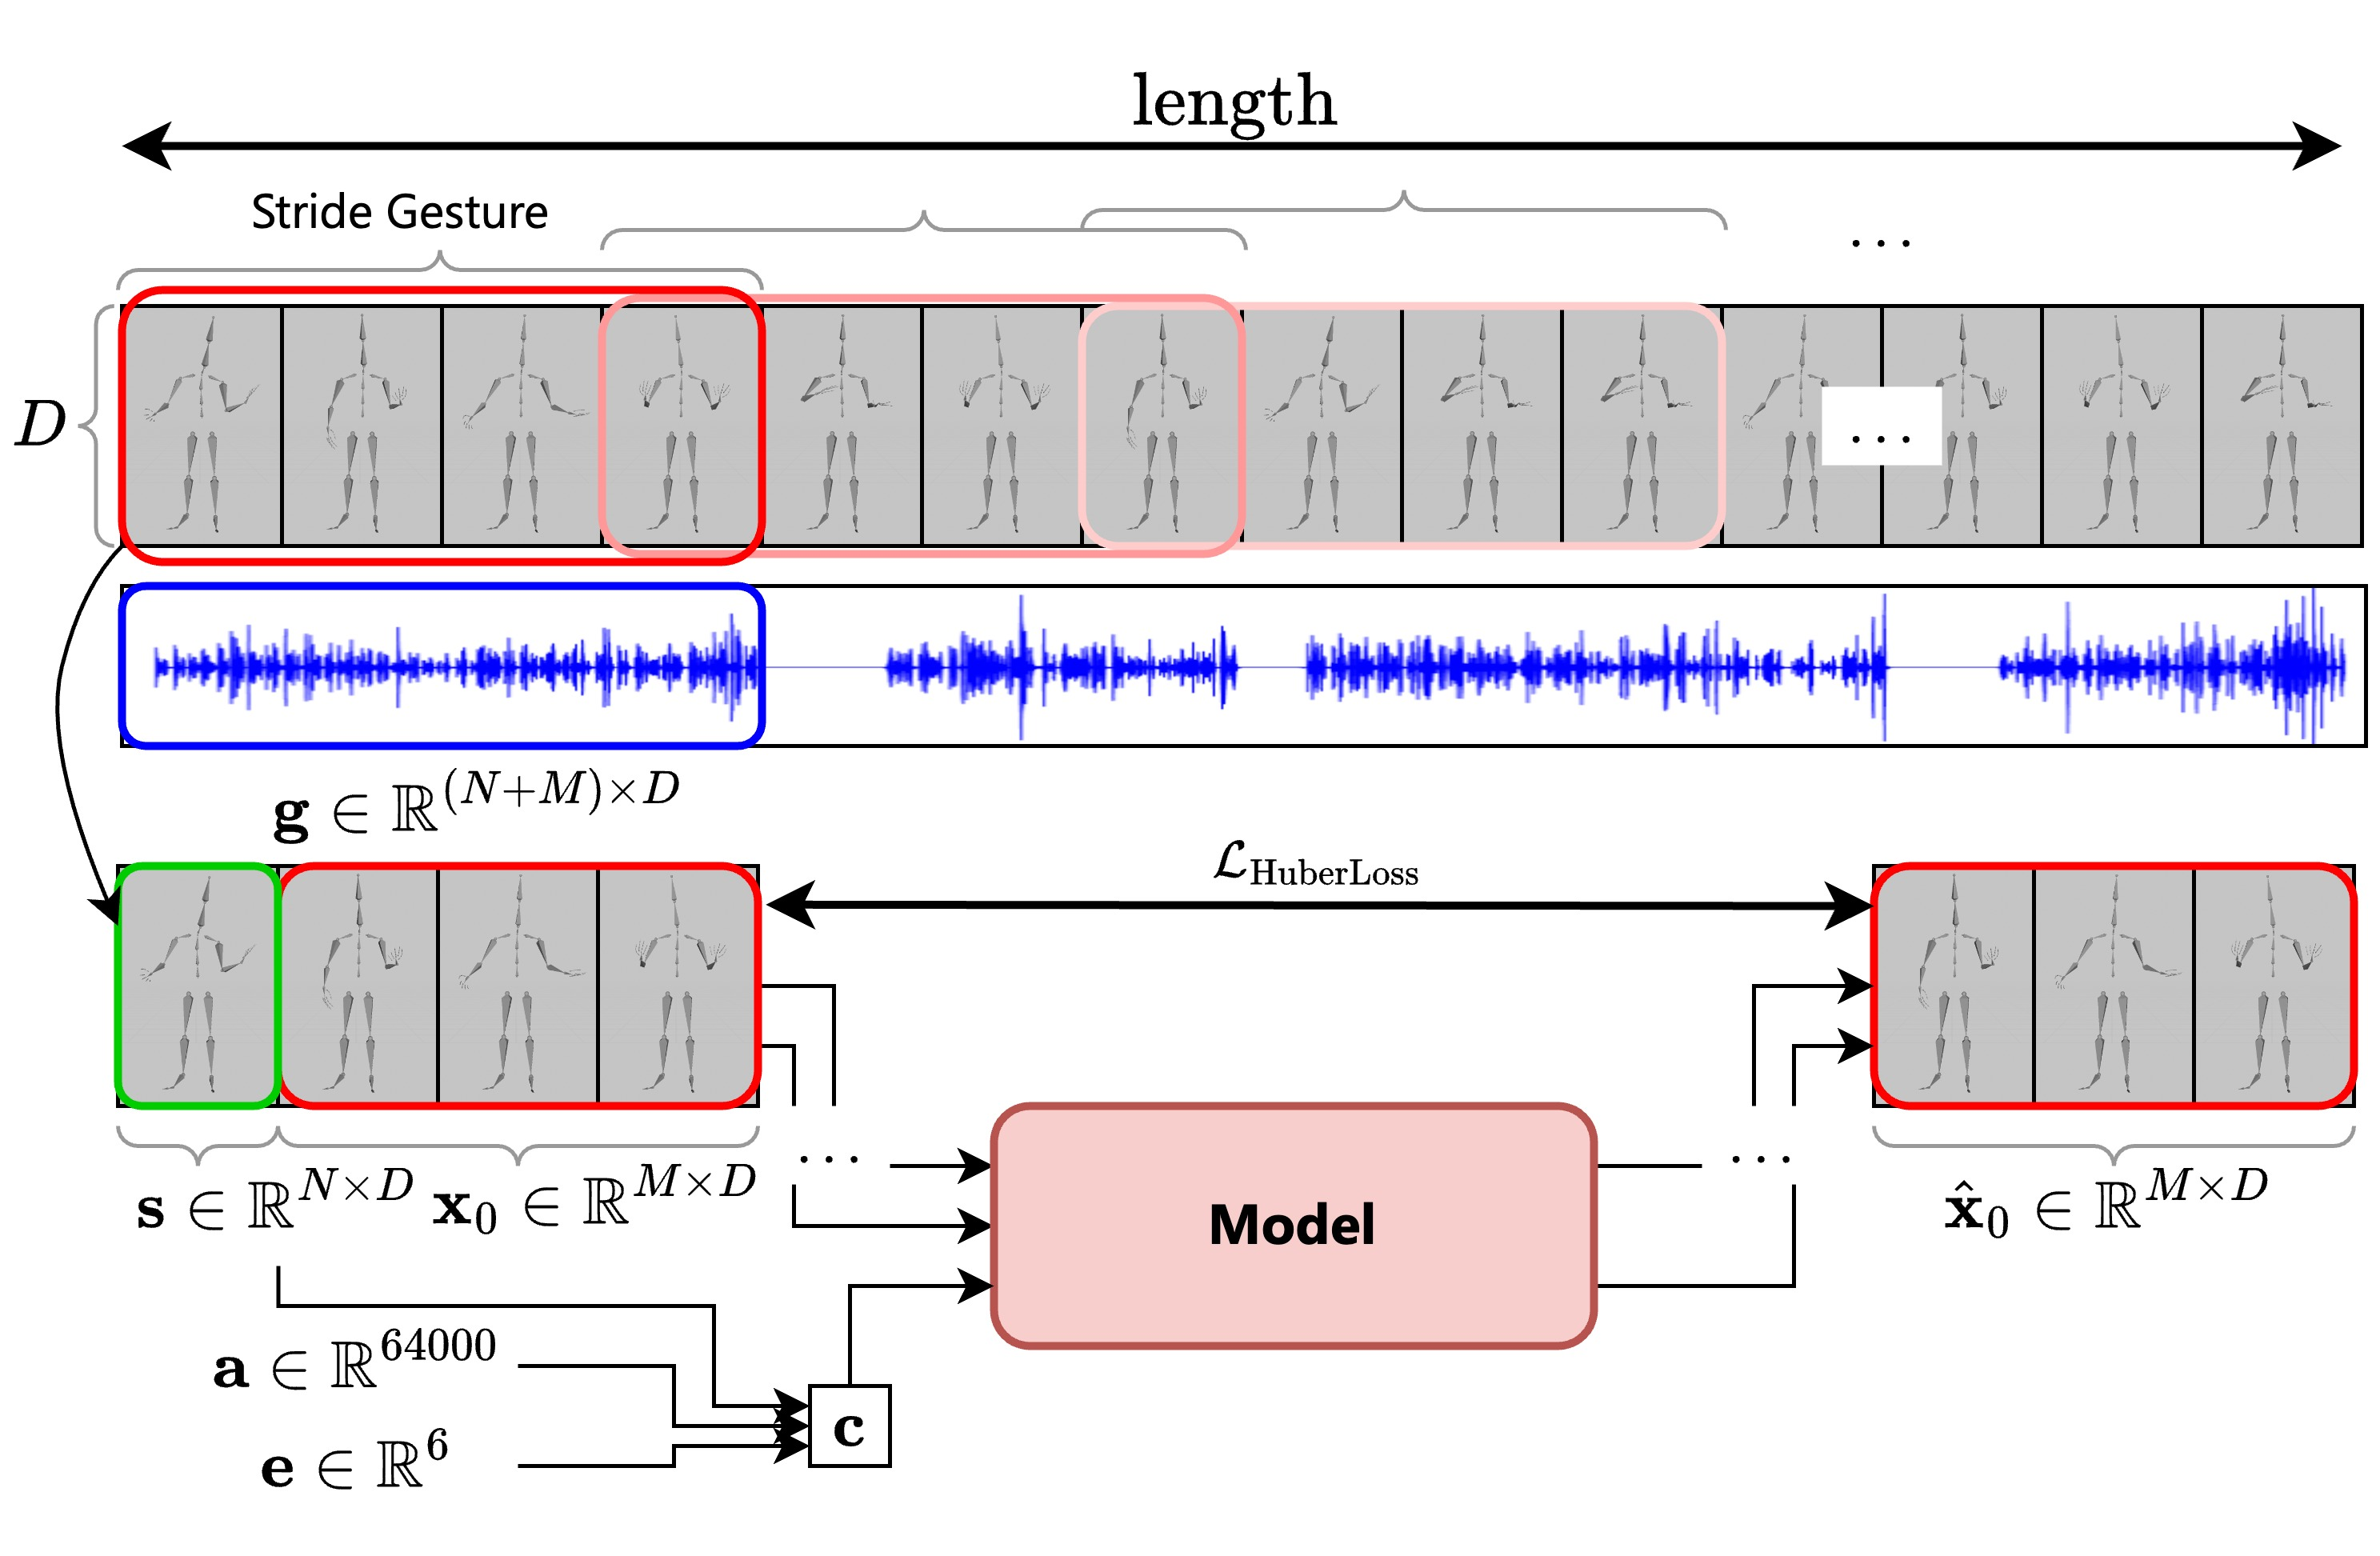
\includegraphics[width=0.8\linewidth]{SequenceGesture.jpg}
%%	\end{figure}
%%	
%	Cho chuỗi cử chỉ $\mathbf{g} \in \mathbb{R}^{(N+ M) \times D}$, với $\mathbf{s} \in \mathbb{R}^{N \times D}$ và đoạn cử chỉ nhãn $\mathbf{x}_0 \in \mathbb{R}^{M \times D}$ với $D=1141$, $N=8$, $M=80$. Chuỗi âm thanh $\mathbf{a} \in \mathbb{R}^{64000}$ (4s: $16000$ sample rate). Cảm xúc $\mathbf{e} \in \mathbb{R}^6$. 
%%	$\{\beta_t \in (0, 1)\}_{t=1}^T$
%
%\end{frame}




\begin{frame}{Tổng quan phương pháp}
	
	\begin{figure}
		\centering
		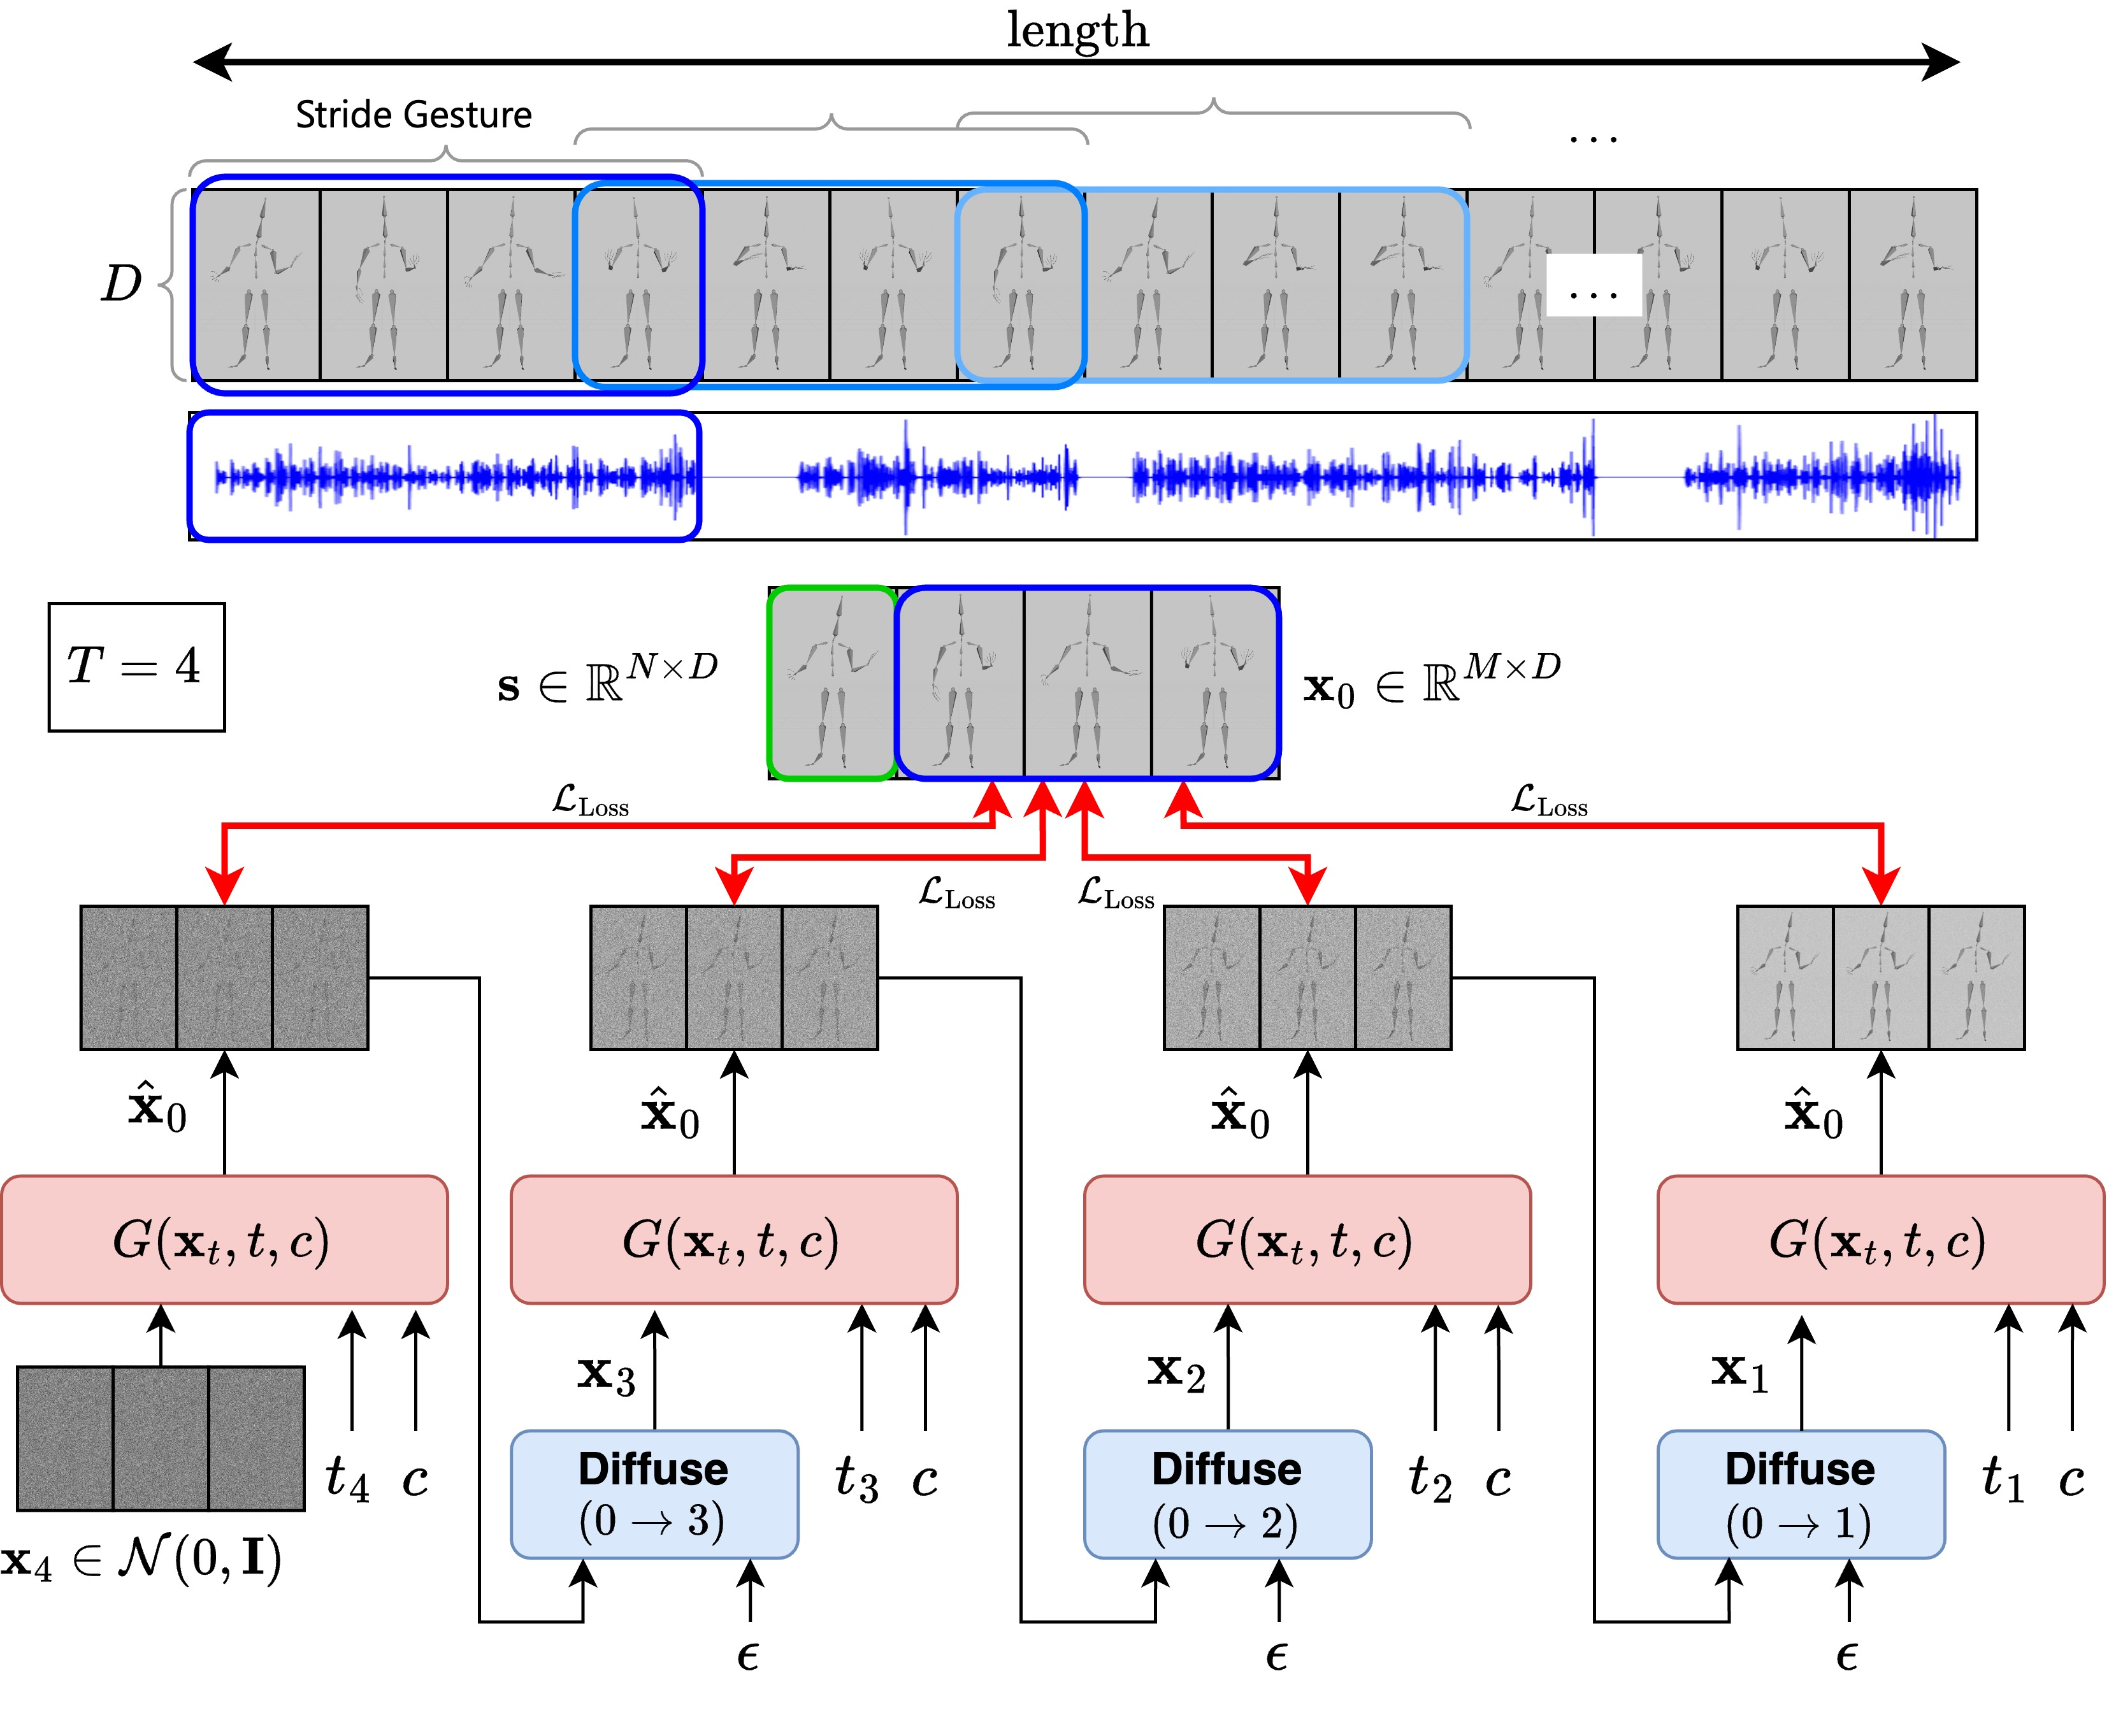
\includegraphics[width=0.9\linewidth]{OverviewArchitecture.jpg}
	\end{figure}
	
\end{frame}

\begin{frame}{Kiến trúc OHGesture}
	\begin{figure}
		\centering
		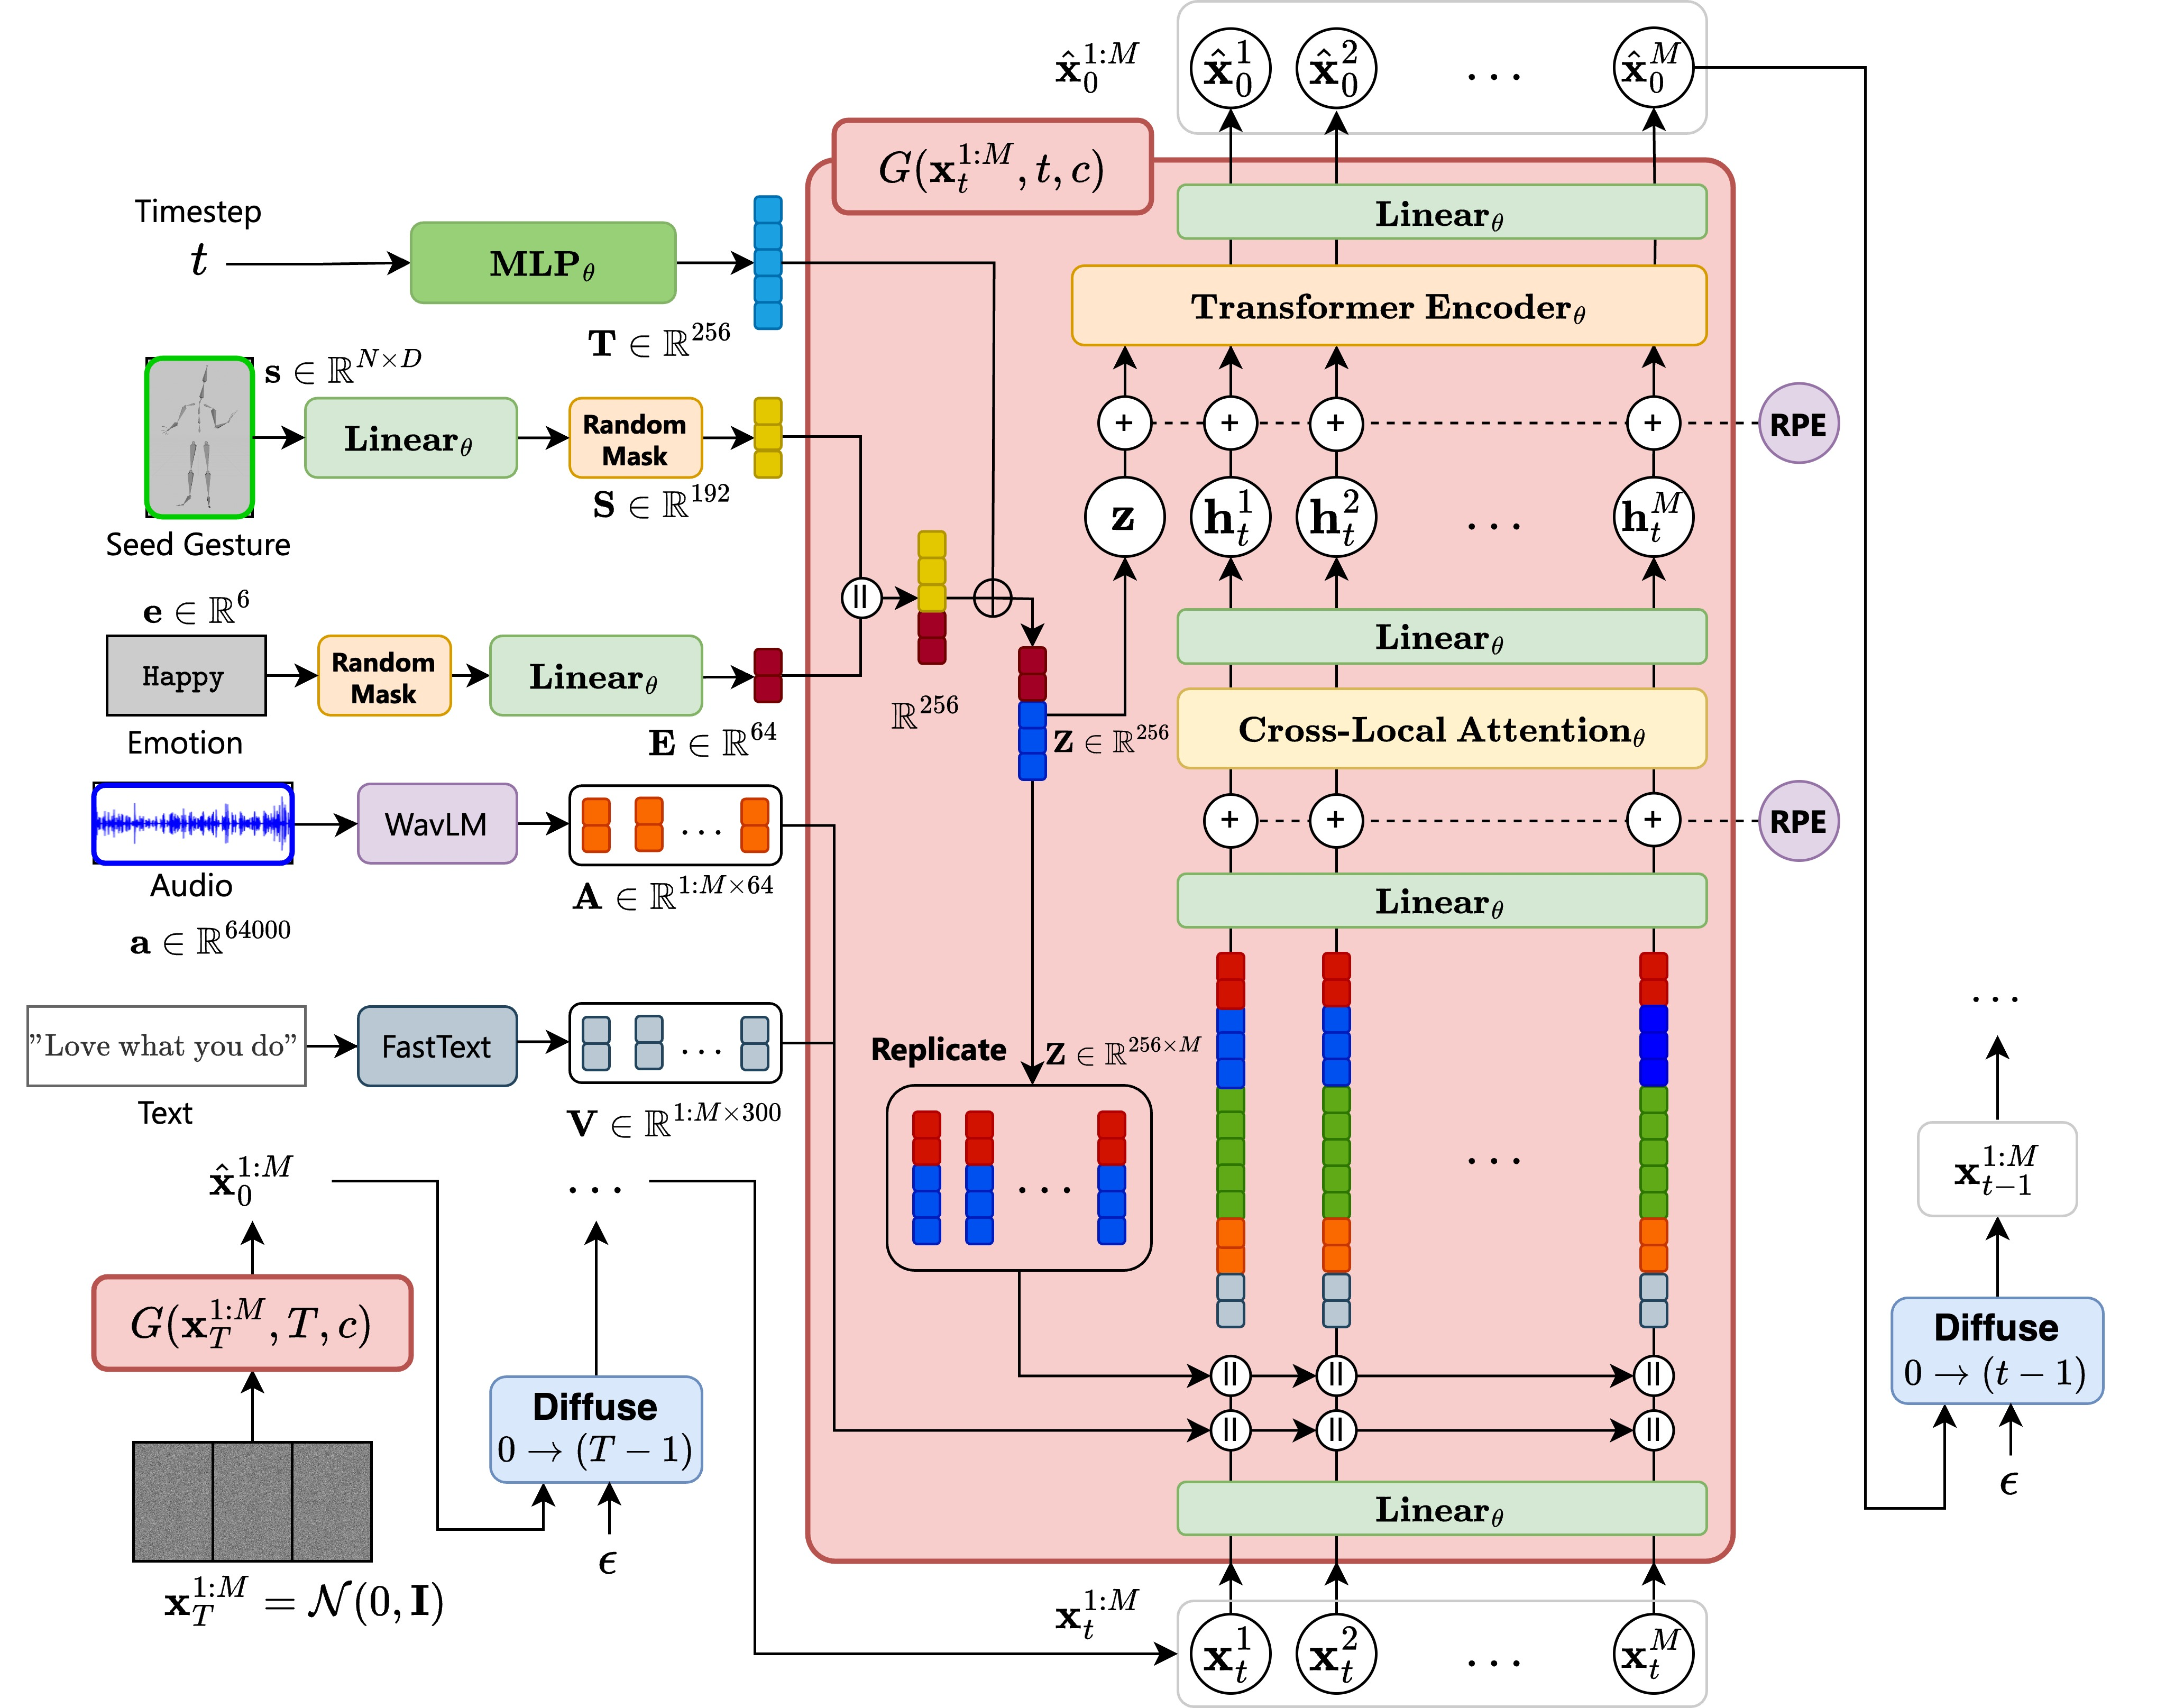
\includegraphics[width=0.9\linewidth]{OHGesture}
	\end{figure}
\end{frame}


\begin{frame}{Cross-Local Attention and Self-Attention}
	\small
	\textbf{Cross-Local Attention}
	\begin{equation*} \label{eq:attention}
		\operatorname{Attention}(\mathbf{Q}, \mathbf{K}, \mathbf{V}, \mathbf{M})=\operatorname{softmax}\left(\frac{\mathbf{Q} \mathbf{K}^{T}+\mathbf{M}}{\sqrt{C}}\right) \mathbf{V}
	\end{equation*}
	

	\begin{columns}
%		Transfomer Encoder : 
		
		\begin{column}{0.5\textwidth}
				\textbf{Self-Attention}
			$$
			f_{\text{MultiHead}(\mathbf{X})} = \operatorname{concat} \left( \mathbf{H}_1, \mathbf{H}_2, \dots, \mathbf{H}_h \right) \mathbf{W}_O
			$$
			
			$$
			\mathbf{H}_i = \operatorname{softmax} \left( \frac{\mathbf{Q}_i \mathbf{K}_i^T}{\sqrt{d_k}} \right) \mathbf{V}_i
			$$
		\end{column}
		
		\begin{column}{0.5\textwidth}
			\begin{figure}
				\centering
				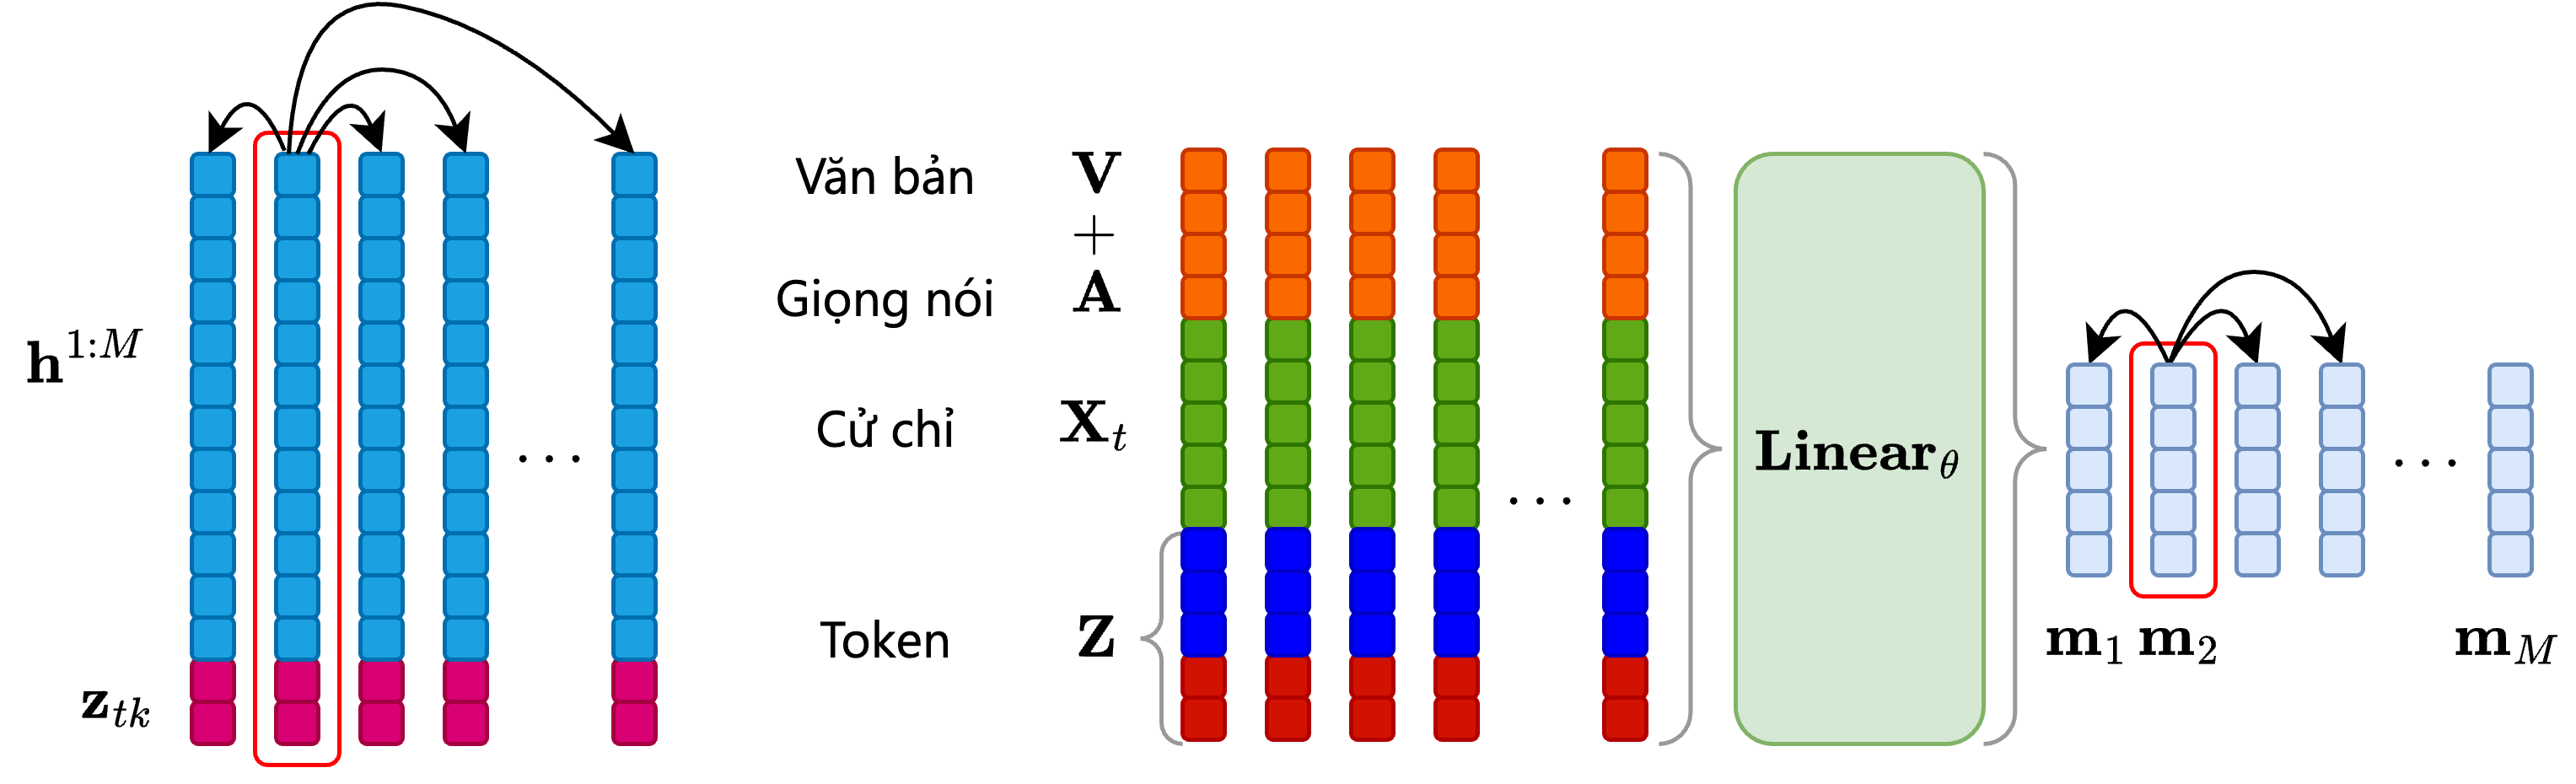
\includegraphics[width=\linewidth]{CrossLocalAttention}
			\end{figure}
		\end{column}
	\end{columns}
	
	
	
\end{frame}



%\begin{frame}{}
%%	Mục tiêu: Áp dụng mô hình Diffusion cho vector tiềm ẩn:
%	1. Forward process:
%	$$
%	x_t = \sqrt{\alpha_t}x_0 + \sqrt{1-\alpha_t}\epsilon, \text{ where } \epsilon \sim \mathcal{N}(0,1)
%	$$
%	
%	2. Model prediction
%	- Input: $x_t$
%	- Output: $\hat{x}_0$ (predicted clean motion)
%	- Conversion between $\hat{x}_0$ and $\hat{\epsilon}$:
%	$$
%	\hat{\epsilon} = \frac{x_t - \sqrt{\alpha_t}\hat{x}_0}{\sqrt{1-\alpha_t}}
%	$$
%	
%	$$\hat{x}_0 = \frac{x_t - \sqrt{1-\alpha_t}\hat{\epsilon}}{\sqrt{\alpha_t}}$$
%	
%	3. Loss
%	$$\mathcal{L} = \| x_0 - \hat{x}_0\|^2 \text{ or } \|\epsilon - \hat{\epsilon}\|^2$$
%
%4. Sampling (Inference):
%	$$x_{t-1} = \sqrt{\alpha_{t-1}}\hat{x}_0 + \sqrt{1-\alpha_{t-1}-\sigma_t^2}\hat{\epsilon} + \sigma_t z$$
%%	\begin{figure}
%%		\centering
%%		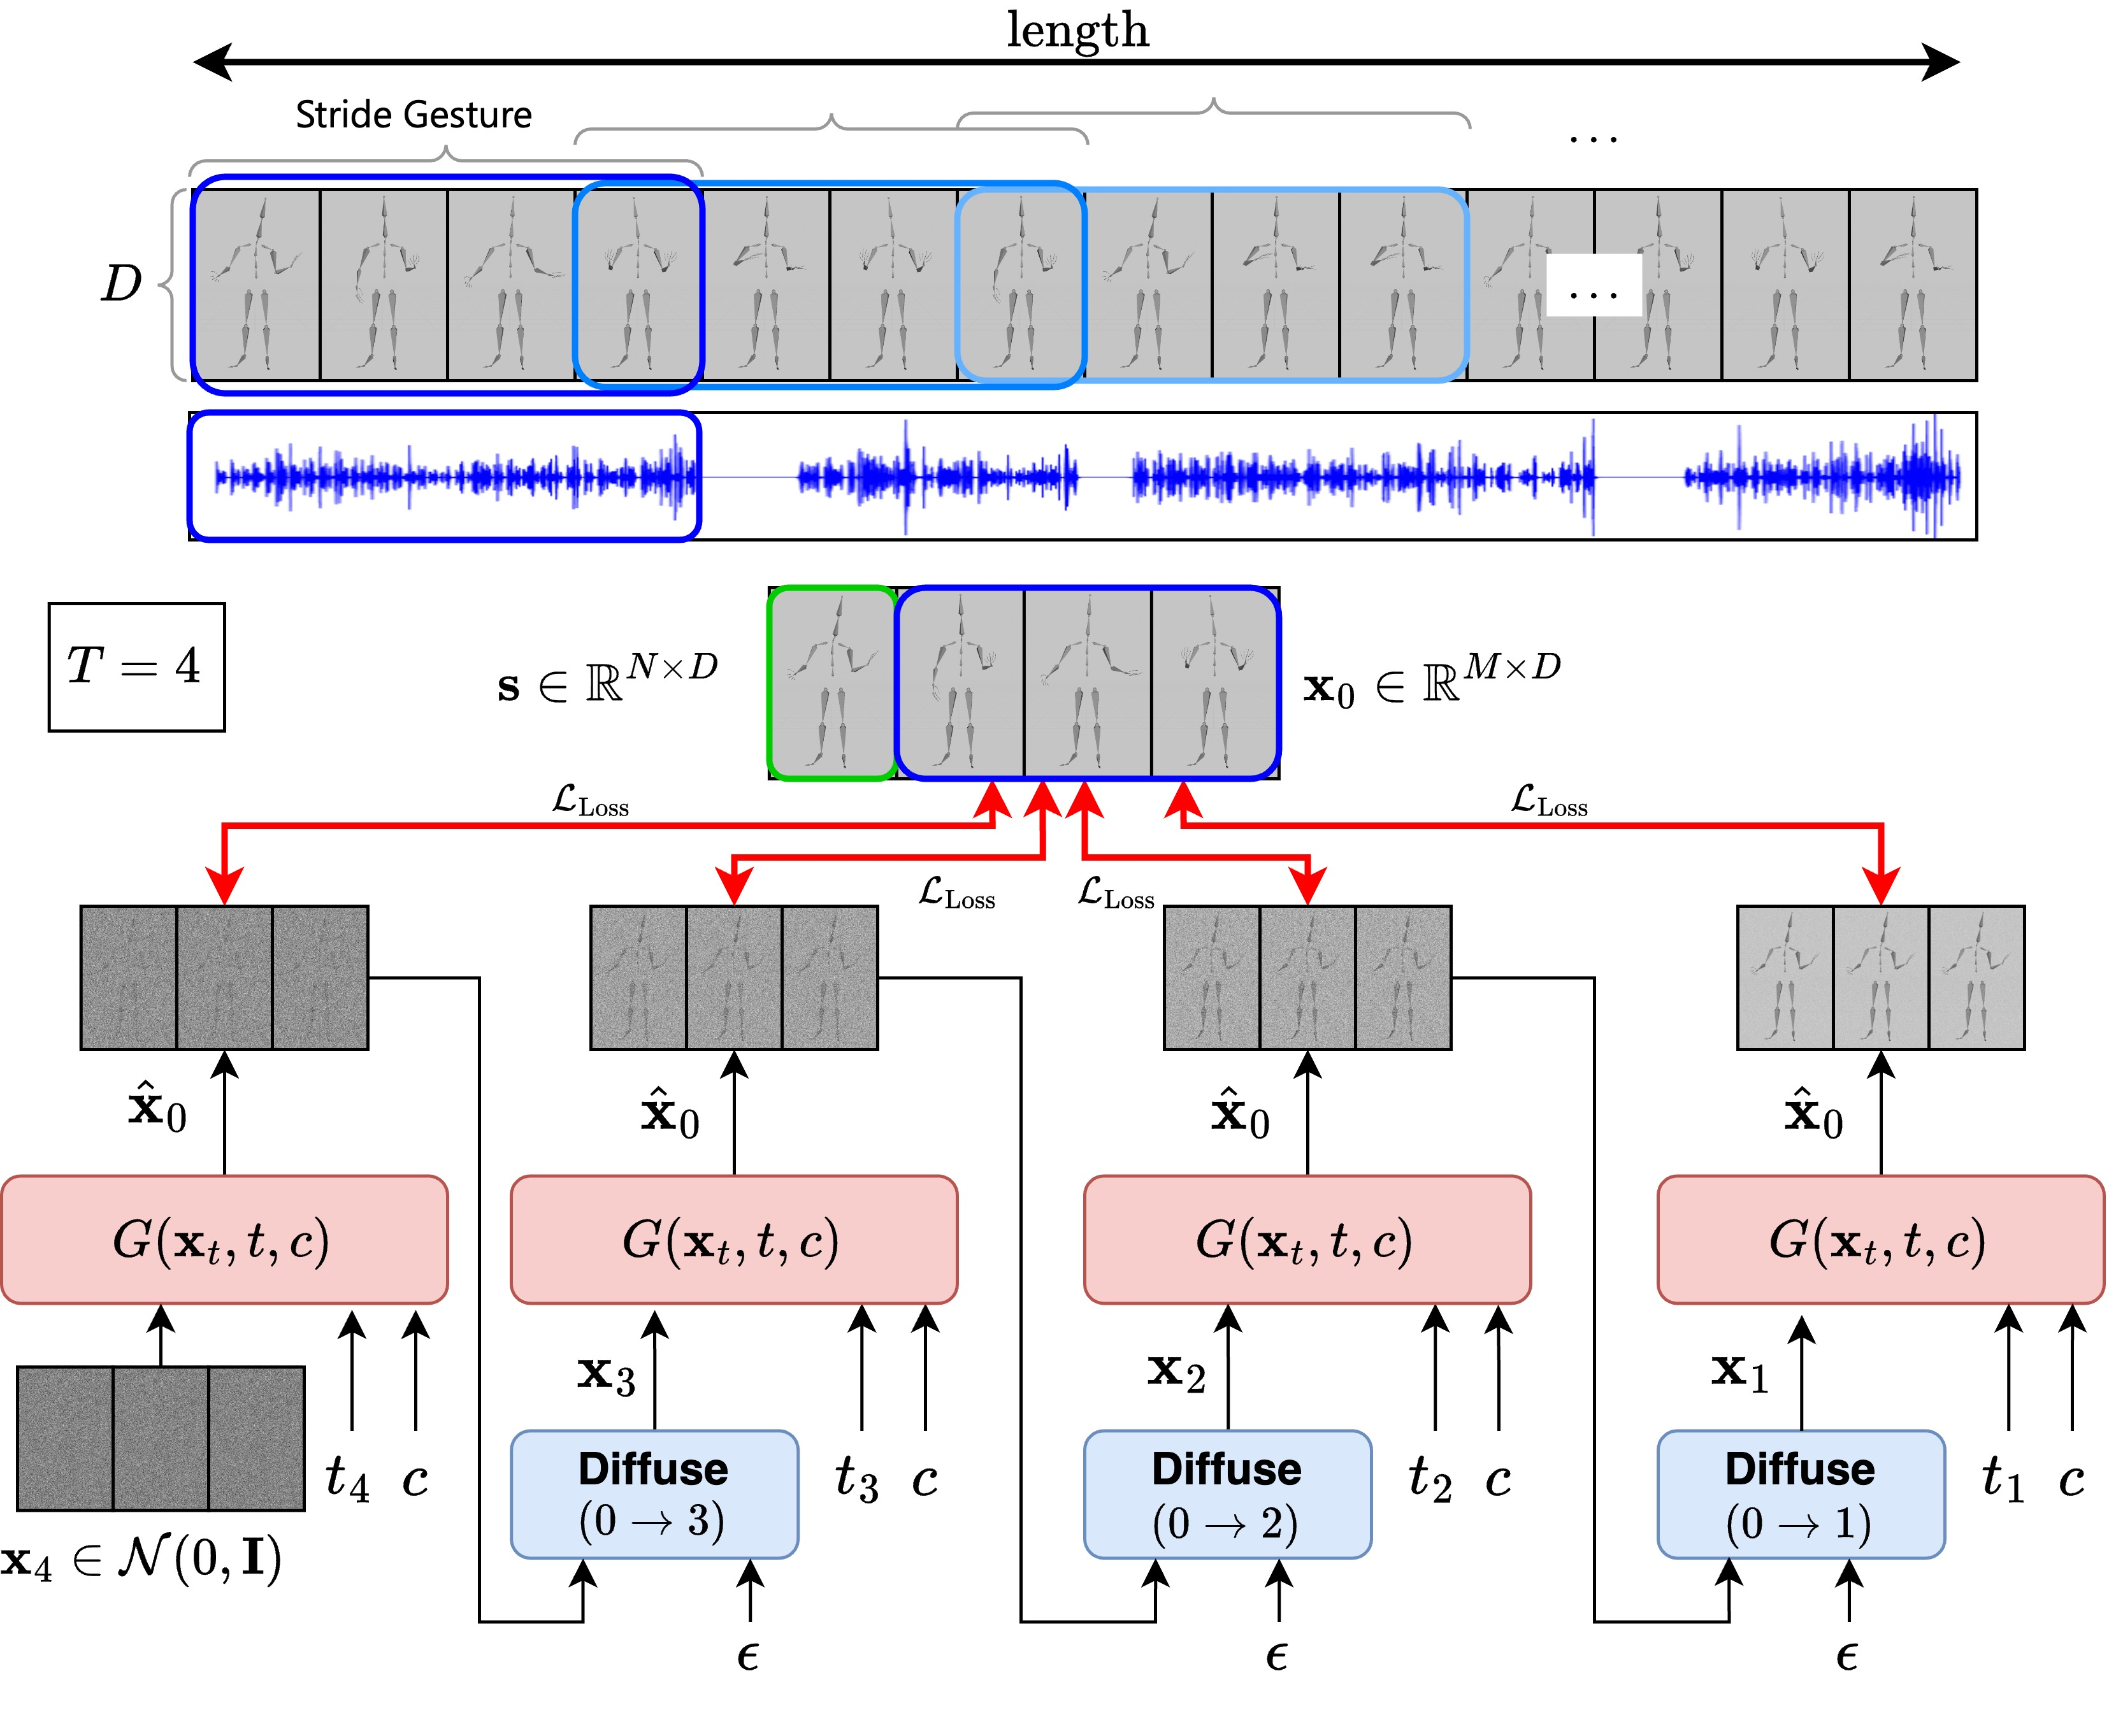
\includegraphics[width=\linewidth]{OverviewArchitecture}
%%	\end{figure}
%	
%\end{frame}
%OverviewConditionDiffusion


\begin{frame}{Emotion-controllable Gesture Generation}
	\begin{equation} \label{eq:condition}
		\hat{\mathbf{x}}_{0} = G \left(\mathbf{x}_{t}, t, c\right)
	\end{equation}
	
	\textbf{Classifier-free guidance}
	\begin{itemize}
		\item Unconditional: $c_1 = [ \varnothing, \varnothing, a ]$
		\item Conditional: $c_1 = [ s, e, a ]$:
	\end{itemize}
	\begin{equation} \label{eq:denoise}
		\hat{\mathbf{x}}_{0 \gamma, c_{1}, c_{2}}=\gamma G \left(\mathbf{x}_{t}, t, c_{1}\right)+(1-\gamma) G \left(\mathbf{x}_{t}, t, c_{2}\right)
	\end{equation}
	Emotion-controllable: $c_1 = [ s, e_1, a ]$, $c_2 = [ s, e_2, a ]$.
	
	\textbf{Huber Loss}
	
	\begin{equation} \label{eq:huberloss}
		\mathcal{L}=E_{\mathbf{x}_{0} \sim q\left(\mathbf{x}_{0} \mid c\right), t \sim[1, T]}\left[\operatorname{HuberLoss}\left(\mathbf{x}_{0}-\hat{\mathbf{x}}_{0}\right)\right]
	\end{equation}
	
	$\mathcal{L}_{\delta}(y, f(x)) = 
	\begin{cases} 
		\frac{1}{2} (y - f(x))^2 & \operatorname{for } |y - f(x)| \leq \delta, \\
		\delta \cdot |y - f(x)| - \frac{1}{2} \delta^2 & \operatorname{otherwise}.
	\end{cases}
	$
	
\end{frame}

%\begin{frame}
%	\begin{figure}
%		\centering
%		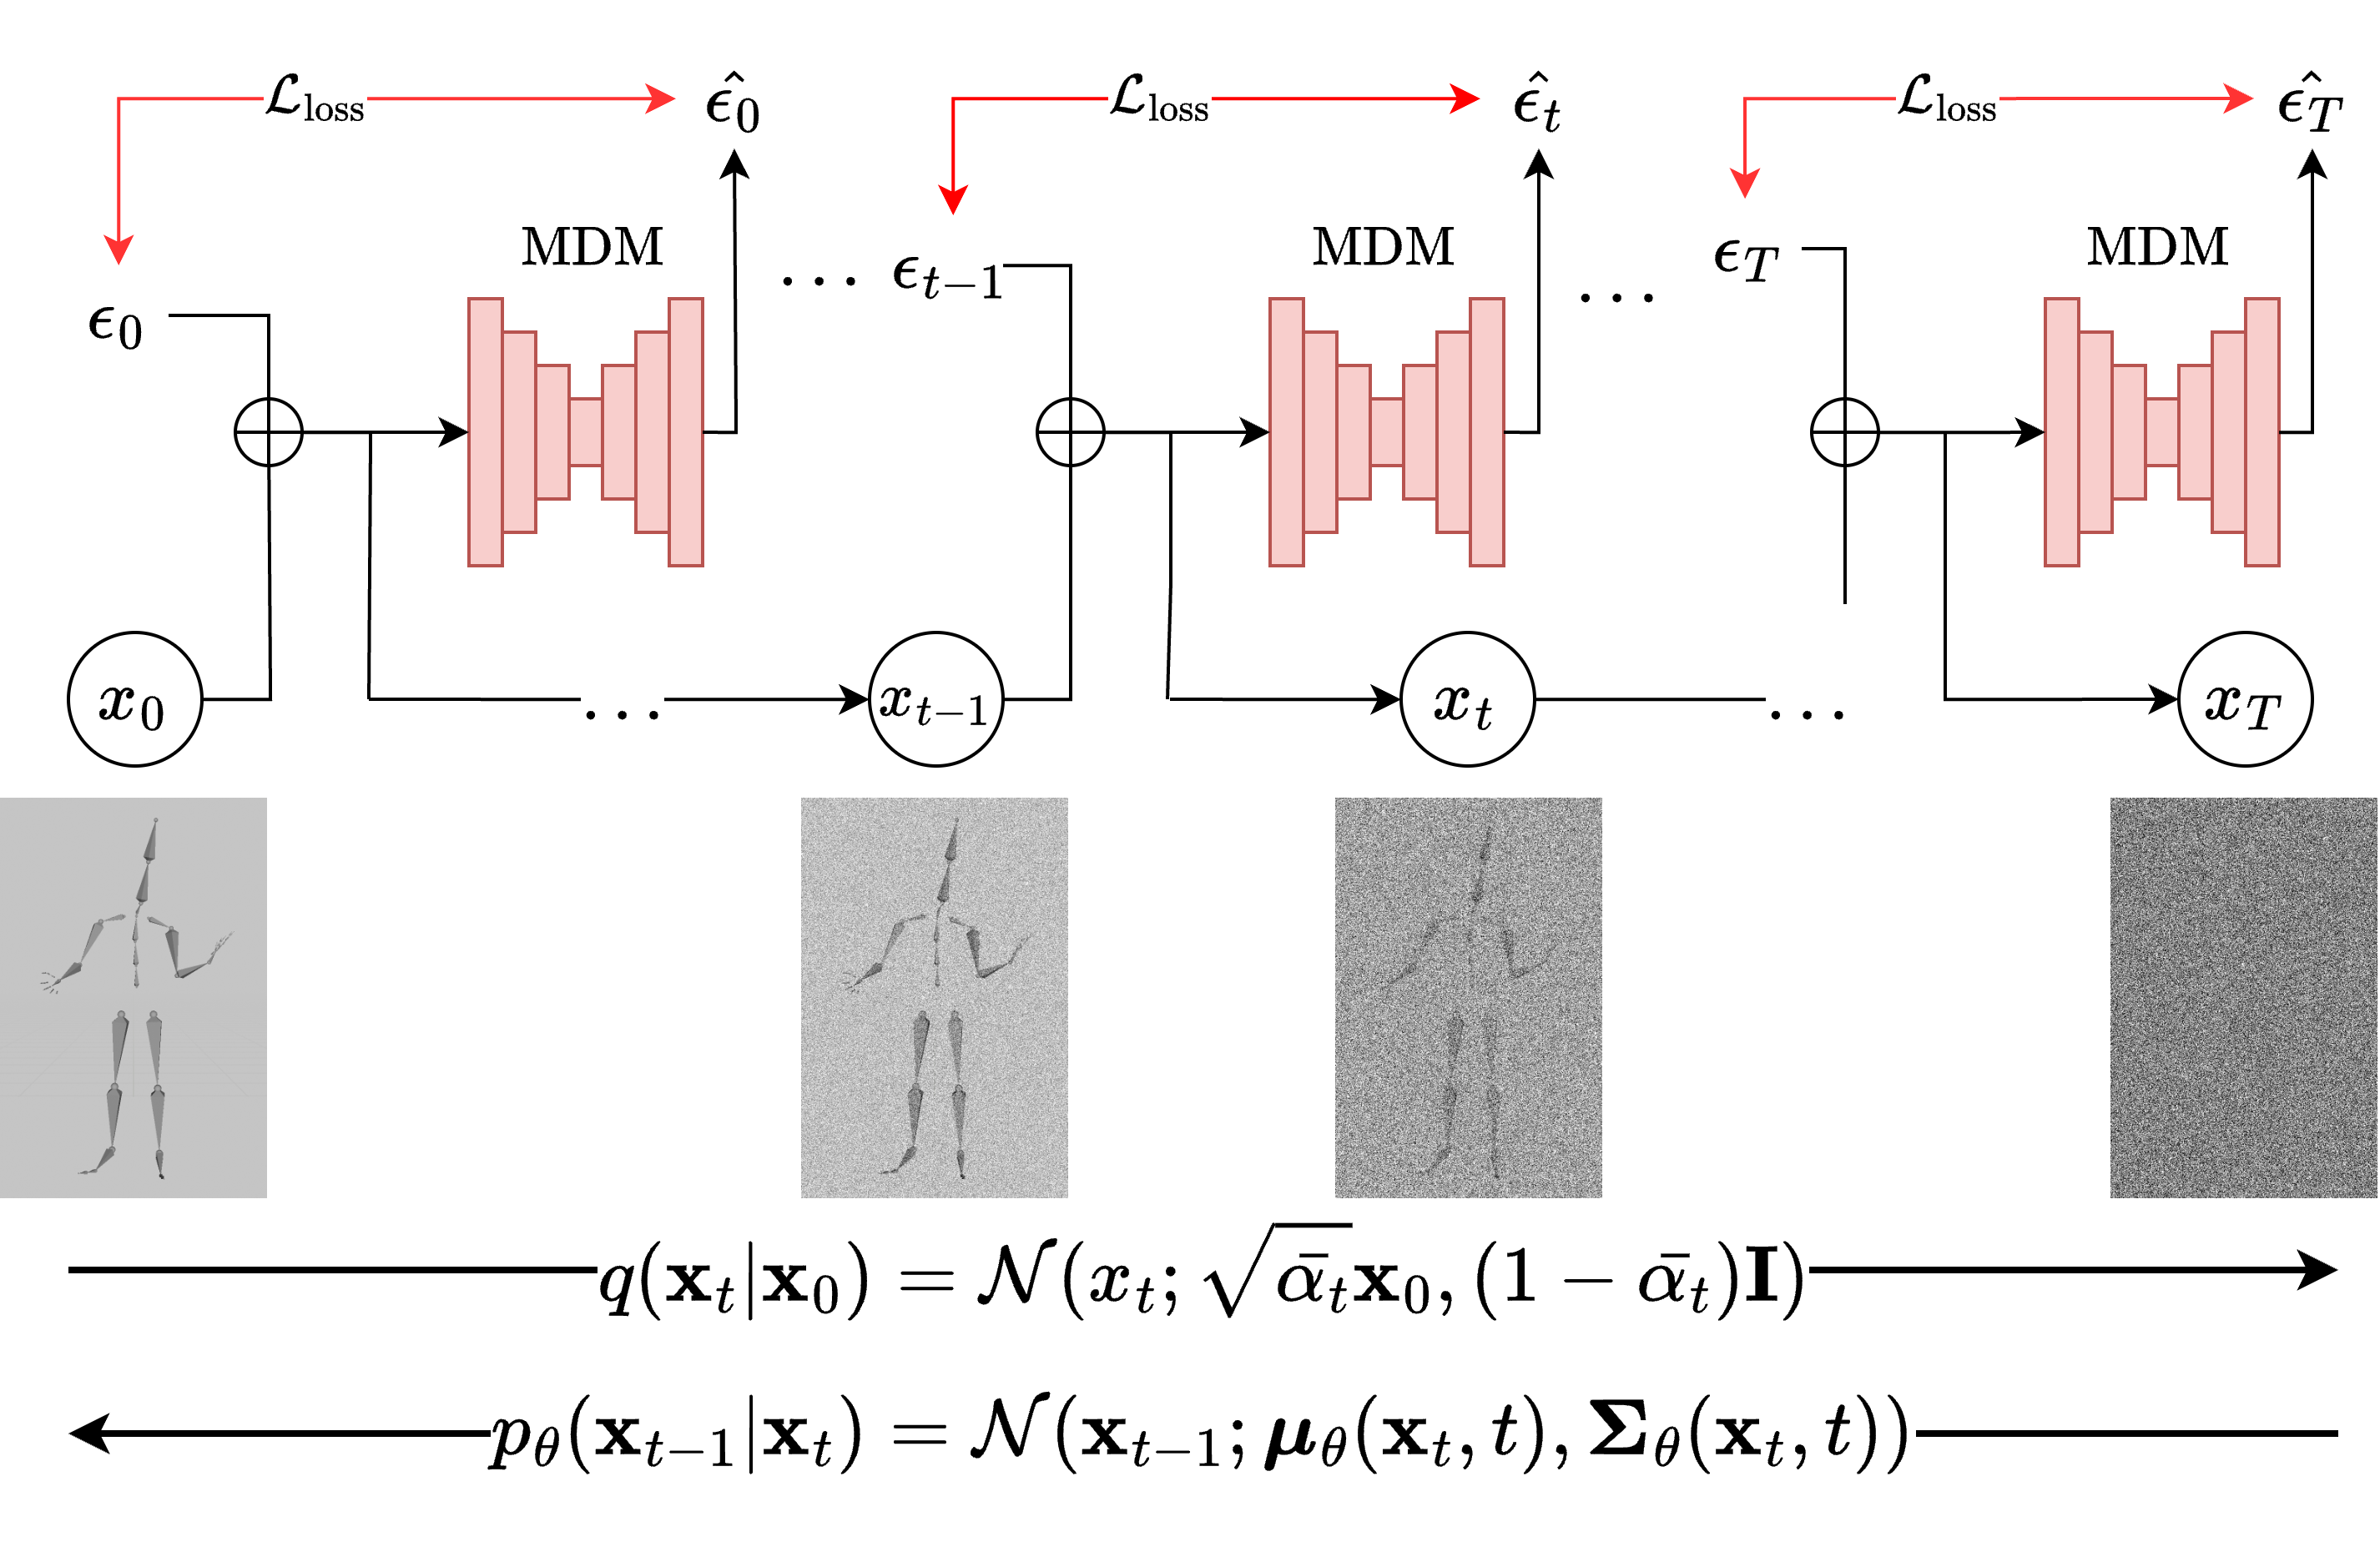
\includegraphics[width=0.8\linewidth]{DiffusionProcess}
%	\end{figure}
%\end{frame}


%\begin{figure} 
%	\centering
%	\includegraphics[width=0.8\linewidth]{DiffusionForward}
%\end{figure}


%\begin{frame}
%	
%	$
%	\label{Gaussian}
%	q\left(x_t \mid x_{t-1}\right)=\mathcal{N}\left(x_t ; \sqrt{1-\beta_t} x_{t-1}, \beta_t \mathbf{I}\right)
%	$
%	
%	$
%	\label{eq1}
%	q\left({x}_{1:T} \mid {x}_0\right)=\prod_{t=1}^T q\left({x}_t \mid {x}_{t-1}\right)
%	$
%	$
%	p_\theta\left({x}_{t-1} \mid {x}_t\right)=\mathcal{N}\left({x}_{t-1} ; {\mu}_\theta\left({x}_t, t\right), {\Sigma}_\theta\left({x}_t, t\right)\right)
%	$
%	
%	$
%	q\left({x}_t \mid {x}_0\right)=\mathcal{N}\left({x}_t ; \sqrt{\bar{\alpha}_t} {x}_0,\left(1-\bar{\alpha}_t\right) \mathbf{I}\right)
%	$
%	
%	$
%	\hat{x}_0=G\left(x_t, t, c\right)
%	$
%\end{frame}

	
%	\begin{columns}
	%		\begin{column}{0.5\textwidth}
		%			\textbf{DDPM (stochastic sampling):}
		%			\begin{itemize}
			%			\item Predict $x_0$ from $x_t$
			%			
			%			\item Convert to $\epsilon_{pred}$
			%			
			%			\item Use the formula:
			%			
			%			$$x_{t-1} = \frac{1}{\sqrt{\alpha_t}} x_t - \frac{1-\alpha_t}{\sqrt{1-\bar{\alpha}t}\sqrt{\alpha_t}} \epsilon_{\text{pred}} + \sigma_t z$$
			%			
			%			\item where $z \sim \mathcal{N}(0,I)$ is random noise
			%			\end{itemize}
		%			
		%		\end{column}
	%		
	%		\begin{column}{0.5\textwidth}
		%			\textbf{DDIM (deterministic sampling):}
		%			
		%			Predict $x_0$ from $x_t$
		%			
		%			NO additional noise term ($\sigma_t = 0$)
		%			
		%			Use the formula:
		%			
		%			$x_{t-1} = \sqrt{\bar{\alpha}{t-1}} x_0^{\text{pred}} + \sqrt{1-\bar{\alpha}_{t-1}} \epsilon_{\text{pred}}$
		%			
		%			Where:
		%			\begin{itemize}
			%			\item $\bar{\alpha}_t$ is the cumulative product of $\alpha$'s from 1 to t
			%			\item $\epsilon_{pred}$ is derived from $x_0$ prediction using:
			%			\item $\epsilon_{pred} = \frac{x_t - \sqrt{\alpha_t}x_{0_{pred}}}{\sqrt{1-\alpha_t}}$
			%			\end{itemize}
		%		\end{column}
	%	\end{columns}
	
